\documentclass{article}

\usepackage[utf8]{inputenc}
\usepackage[brazil]{babel}

\title{Avaliação de Reconhecimento de Padrões}
\author{Rúbia Reis Guerra \\ 2013031143}

\usepackage{Sweave}
\begin{document}
\Sconcordance{concordance:prova.tex:prova.Rnw:%
1 8 1 1 0 4 1 1 2 1 0 6 1 1 11 13 0 1 2 1 1 1 2 1 0 6 1 1 3 5 0 1 2 1 1 %
1 2 1 0 5 1 9 0 1 1 4 0 1 2 1 1 1 6 5 0 1 1 1 5 8 0 1 2 1 1 1 6 5 0 1 1 %
1 5 8 0 1 2 3 1 1 4 3 0 4 1 7 0 2 2 7 0 1 2 1 4 3 0 1 5 4 0 1 1 24 0 1 %
2 8 1 1 4 3 0 1 1 4 0 1 2 3 1 1 2 1 0 6 1 1 2 1 4 3 0 1 9 6 0 1 1 30 0 %
1 2 2 1 1 2 1 0 6 1 1 2 1 4 3 0 1 9 6 0 1 1 30 0 1 2 2 1}

\maketitle

\section{Pacotes utilizados}
\begin{Schunk}
\begin{Sinput}
> rm(list=ls())
> library('MASS')
> library('mlbench')
> library('mclust')
> library('stats')
> library('kernlab')
> library('caret')
> ###########################
> # F-Score #
> fscore <- function(X,c1,c2,n){
+   f <- c()
+   for(i in 1:n)
+   {
+     f[i] <- ((mean(c1[,i]) - mean(X[,i]))^2
+              +(mean(c2[,i]) - mean(X[,i]))^2)/(sd(c1[,i])^2+sd(c2[,i])^2)
+   }
+   return(f)
+ }
\end{Sinput}
\end{Schunk}

\section{Base de Dados}
\begin{Schunk}
\begin{Sinput}
> bupa <- as.matrix(read.csv("bupa.data", header=FALSE))
> X <- bupa[,(1:6)] # dados de entrada
> Y <- as.matrix(2*(bupa[,7]-1.5)) # rotulos das classes como [-1,+1]
> i_cm1 <- which(Y == -1) # amostras da classe -1
> i_c1 <- which(Y == 1) # amostras da classe +1
> Nm1 <- length(i_cm1) # tamanho da classe -1
> N1 <- length(i_c1) # tamanho da classe +1
> ## Plot por pares
> clPairs(bupa, Y)
\end{Sinput}
\end{Schunk}
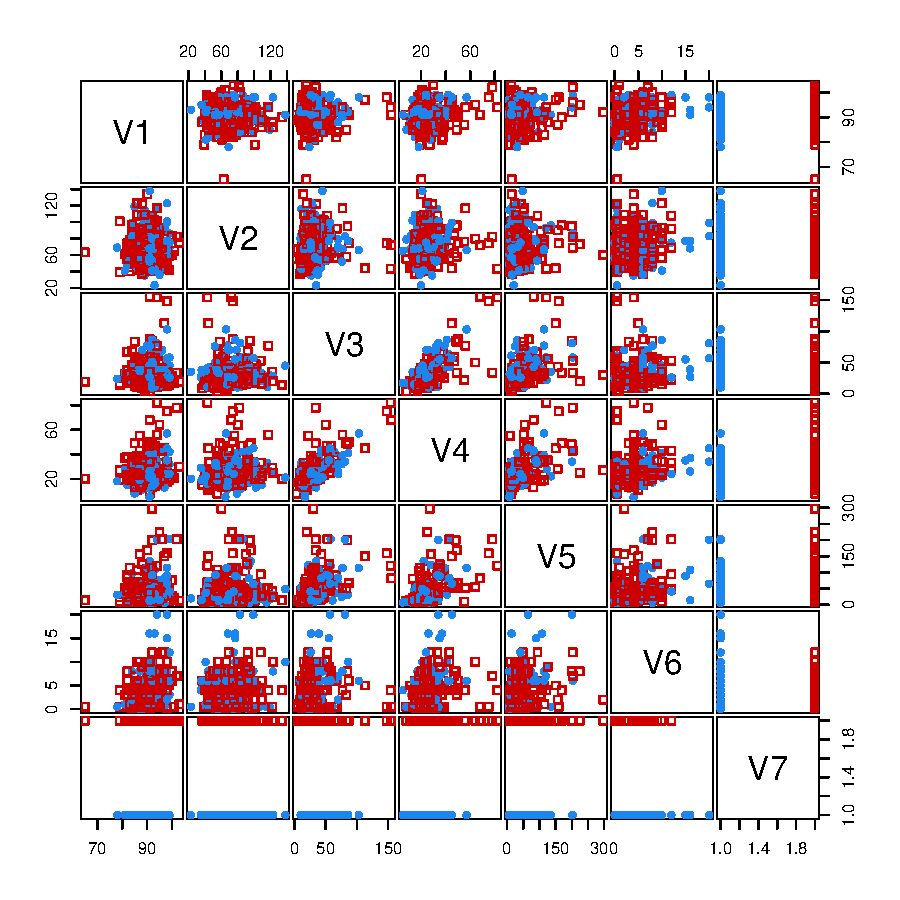
\includegraphics{prova-002}

\section{Análise de Componentes Principais (PCA)}
\begin{Schunk}
\begin{Sinput}
> meanx <- colMeans(X)
> Xrep <- X - t(replicate(dim(X)[1],meanx))
> pcaX <- prcomp(Xrep)
> us <- pcaX$rotation
> projX <- Xrep %*% us
> summary(pcaX)
\end{Sinput}
\begin{Soutput}
Importance of components:
                           PC1     PC2     PC3    PC4    PC5     PC6
Standard deviation     41.2824 18.1518 17.0564 6.1452 4.4264 2.91784
Proportion of Variance  0.7129  0.1378  0.1217 0.0158 0.0082 0.00356
Cumulative Proportion   0.7129  0.8508  0.9724 0.9882 0.9964 1.00000
\end{Soutput}
\begin{Sinput}
> barplot(pcaX$sdev)
\end{Sinput}
\end{Schunk}
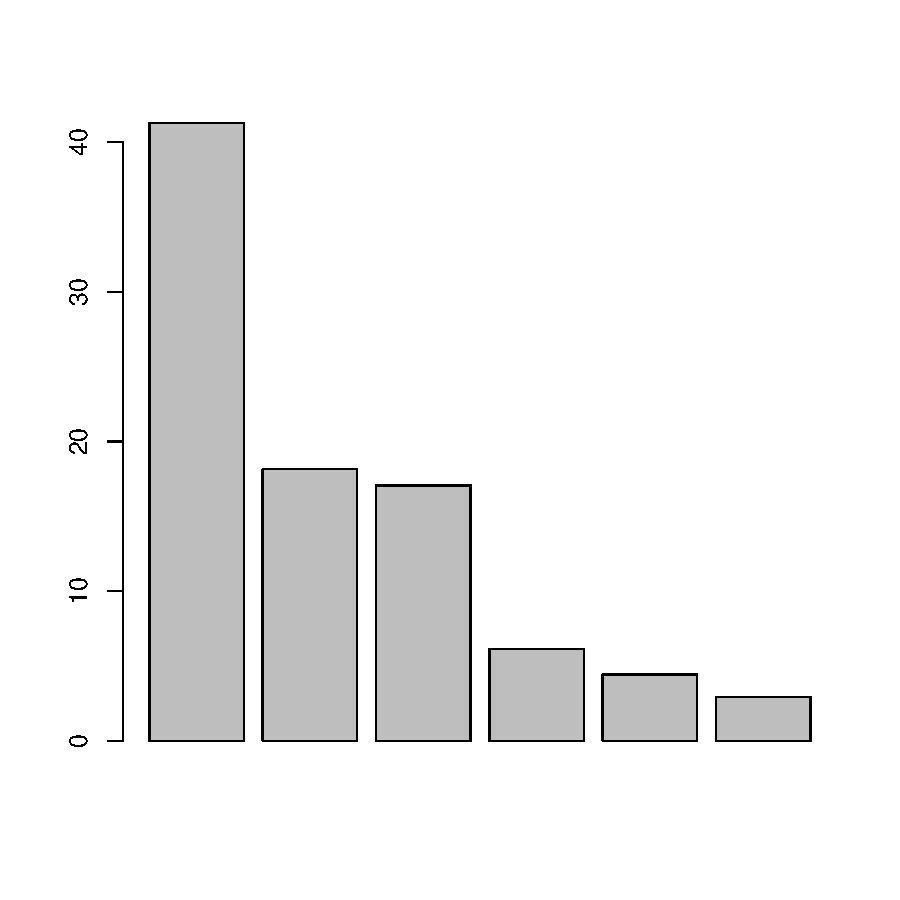
\includegraphics{prova-003}

A partir dos autovalores encontrados para o dataset \textit{bupa}, observamos que as três primeiras coordenadas concentram a maior parte da varância dos dados.
\begin{Schunk}
\begin{Sinput}
> # Reduzindo para os dois primeiros eixos
> plot(projX[,1],projX[,2],type='p',
+      xlim=c(min(projX[,1]),max(projX[,1])),
+      ylim=c(min(projX[,2]),max(projX[,2])),
+      xlab='PCA1',ylab='PCA2',col='blue')
> par(new=TRUE)
> plot(projX[which(Y==1),1],projX[which(Y==1),2],type='p',
+      xlim=c(min(projX[,1]),max(projX[,1])),
+      ylim=c(min(projX[,2]),max(projX[,2])),
+      col='red',xlab='PCA1',ylab='PCA2',
+      sub='Projeção das classes em PCA1 e PCA2')
\end{Sinput}
\end{Schunk}
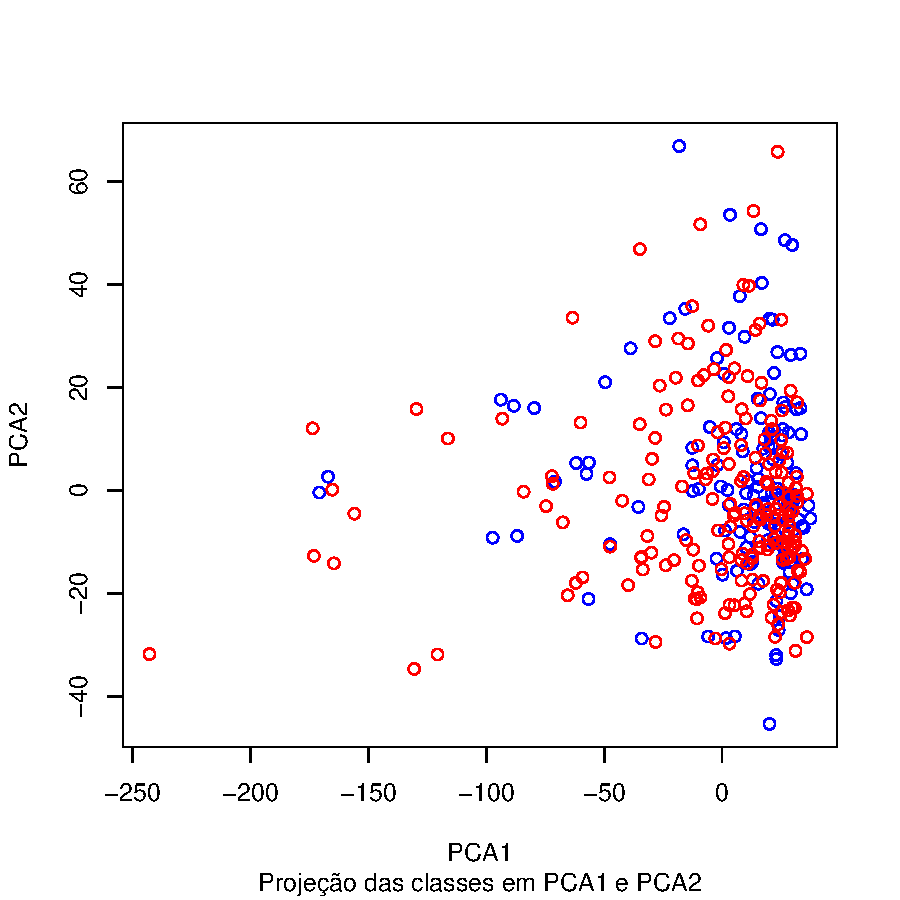
\includegraphics{prova-004}

Em contrapartida, as cordenadas 4 a 6 pouco representam a variância do dataset. Pode-se observar uma maior sobreposição das classes na projeção abaixo:
\begin{Schunk}
\begin{Sinput}
> # Comparacao: reduzindo aos eixos 4 e 5
> plot(projX[,4],projX[,5],type='p',
+      xlim=c(min(projX[,4]),max(projX[,4])),
+      ylim=c(min(projX[,5]),max(projX[,5])),
+      xlab='PCA4',ylab='PCA5',col='blue')
> par(new=TRUE)
> plot(projX[which(Y==1),4],projX[which(Y==1),5],type='p',
+      xlim=c(min(projX[,4]),max(projX[,4])),
+      ylim=c(min(projX[,5]),max(projX[,5])),col='red',
+      xlab='PCA4',ylab='PCA5',
+      sub='Projeção das classes em PCA4 e PCA5')
\end{Sinput}
\end{Schunk}
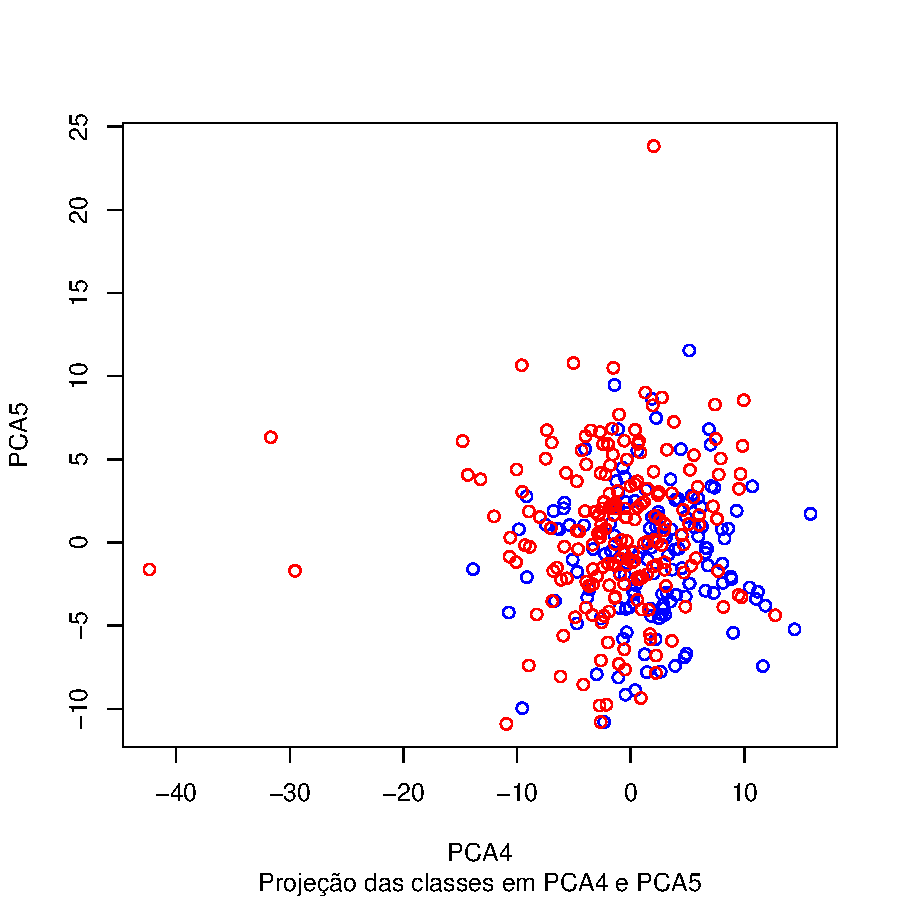
\includegraphics{prova-005}

\section{Seleção de Características}
Para identificar as características da base \textit{bupa} que melhor representam a variância dos dados, podemos comparar os resultados obtidos por meio de F-score e clustering (kmeans e clustering hierárquico), e, então inferir a importância dos atributos.
\subsection{F-Score}
\begin{Schunk}
\begin{Sinput}
> ###########################
> # F-Score #
> c1 <- X[which(Y==-1),]
> c2 <- X[which(Y==1),]
> n <- dim(X)[2]
> f <- fscore(X,c1,c2,n)
> print(f)
\end{Sinput}
\begin{Soutput}
[1] 0.0090474857 0.0101072589 0.0013483365 0.0280948506 0.0237967908
[6] 0.0004832165
\end{Soutput}
\end{Schunk}
Ordenando os atributos pelo grau de concentração de variância dos dados:
\begin{Schunk}
\begin{Sinput}
> colnames(X[,order(f)])
\end{Sinput}
\begin{Soutput}
[1] "V6" "V3" "V1" "V2" "V5" "V4"
\end{Soutput}
\end{Schunk}
\subsection{K-Means}
\begin{Schunk}
\begin{Sinput}
> ###########################
> # Kmeans # 
> k <- list()
> for(i in 1:(nrow(t(X))-1))
+ {
+   h <- kmeans(t(X),i)
+   k[[i]] <- h$cluster
+ }
> k
\end{Sinput}
\begin{Soutput}
[[1]]
V1 V2 V3 V4 V5 V6 
 1  1  1  1  1  1 

[[2]]
V1 V2 V3 V4 V5 V6 
 1  1  2  2  2  2 

[[3]]
V1 V2 V3 V4 V5 V6 
 3  3  1  1  2  1 

[[4]]
V1 V2 V3 V4 V5 V6 
 2  2  4  4  3  1 

[[5]]
V1 V2 V3 V4 V5 V6 
 4  4  3  5  1  2 
\end{Soutput}
\end{Schunk}
Observando a mudança de agrupamentos a medida que o número de clusters cresce, podemos inferir que:
\begin{itemize}
\item Os atributos V1 e V2 encontram-se mais próximos, espacialmente, e distantes dos demais;
\item Os atributos V3 e V4 encontram-se mais próximos, espacialmente;
\item No grupo V3 a V5, V5 encontram-se mais afastado dos demais;
\end{itemize}
Assim, podemos simplificar a base, eliminando caracterísitcas que pouco representam os dados (por exemplo, V1 e V3, mantendo-se V2 e V4).
\subsection{Clustering Hierárquico}
Os resultados obtidos por K-Means podem ser melhor observados no dendograma obtido a partir do clustering hierárquico abaixo:
\begin{Schunk}
\begin{Sinput}
> ###########################
> # Hierarchical clustering #
> clusters <- hclust(dist(t(X)))
> plot(clusters)
\end{Sinput}
\end{Schunk}
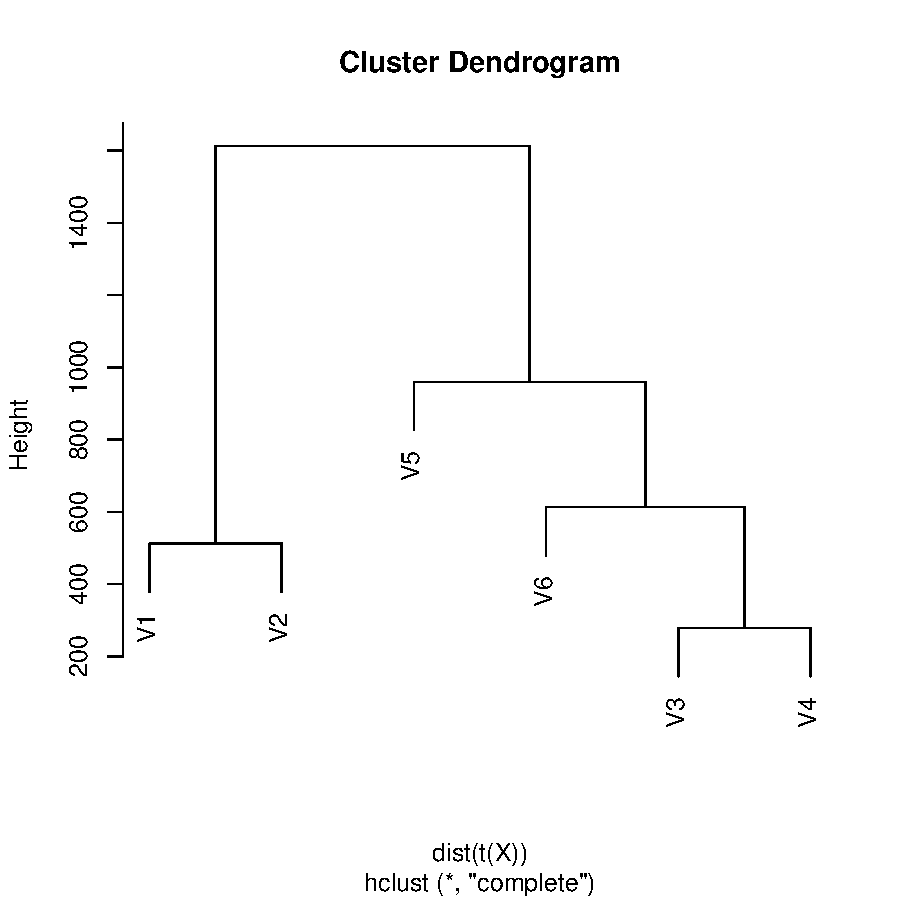
\includegraphics{prova-009}
Observa-se a proximidade dos atributos V1 e V2, em contraste com o grupo V3 a V5, e as similaridades intra-atributos, conforme mencionado na seção anterior.

\section{SVM}
Utilizando a base de dados fornecida, sem realizar seleção ou extração de características, obtem-se:
\begin{Schunk}
\begin{Sinput}
> levels <- unique(Y) 
> Y <- factor(Y, labels=make.names(levels))
> trainIndex <- createDataPartition(bupa[,7],p=.7,list=FALSE)
> trainData <- X[trainIndex,]
> testData  <- X[-trainIndex,]
> trainLabels <- Y[trainIndex]
> testLabels <- Y[-trainIndex]
> set.seed(1492)
> ctrl <- trainControl(method="repeatedcv",
+                      repeats=5,
+                      summaryFunction=twoClassSummary,
+                      classProbs=TRUE)
> svm.tune <- train(x=trainData,
+                   y=trainLabels,
+                   method = "svmRadial",
+                   tuneLength = 9,
+                   preProc = c("center","scale"),
+                   metric="ROC",
+                   trControl=ctrl)
> svm.tune
\end{Sinput}
\begin{Soutput}
Support Vector Machines with Radial Basis Function Kernel 

242 samples
  6 predictor
  2 classes: 'X.1', 'X1' 

Pre-processing: centered (6), scaled (6) 
Resampling: Cross-Validated (10 fold, repeated 5 times) 
Summary of sample sizes: 217, 218, 218, 218, 218, 218, ... 
Resampling results across tuning parameters:

  C      ROC        Sens       Spec     
   0.25  0.6946063  0.5066667  0.8035238
   0.50  0.7030519  0.4757778  0.8500000
   1.00  0.7122751  0.4917778  0.8303810
   2.00  0.7147619  0.4857778  0.8304762
   4.00  0.7027767  0.4742222  0.8359048
   8.00  0.7024720  0.4557778  0.8513333
  16.00  0.6987640  0.4313333  0.8419048
  32.00  0.6747608  0.3677778  0.8616190
  64.00  0.6453471  0.2722222  0.8685714

Tuning parameter 'sigma' was held constant at a value of 0.2502301
ROC was used to select the optimal model using  the largest value.
The final values used for the model were sigma = 0.2502301 and C = 2.
\end{Soutput}
\end{Schunk}
Para as condições dadas, encontrou-se o melhor resultado para C = 2.

Utilizando os resultados conforme a análise de componentes principais, obtem-se:
\begin{Schunk}
\begin{Sinput}
> levels <- unique(Y) 
> Y <- factor(Y, labels=make.names(levels))
> trainIndex <- createDataPartition(bupa[,7],p=.7,list=FALSE)
> trainData <- projX[trainIndex,]
> testData  <- projX[-trainIndex,]
> trainLabels <- Y[trainIndex]
> testLabels <- Y[-trainIndex]
> set.seed(1492)
> ctrl <- trainControl(method="repeatedcv",
+                      repeats=5,
+                      summaryFunction=twoClassSummary,
+                      classProbs=TRUE)
> svm.tune <- train(x=trainData,
+                   y=trainLabels,
+                   method = "svmRadial",
+                   tuneLength = 9,
+                   preProc = c("center","scale"),
+                   metric="ROC",
+                   trControl=ctrl)
> svm.tune
\end{Sinput}
\begin{Soutput}
Support Vector Machines with Radial Basis Function Kernel 

242 samples
  6 predictor
  2 classes: 'X.1', 'X1' 

Pre-processing: centered (6), scaled (6) 
Resampling: Cross-Validated (10 fold, repeated 5 times) 
Summary of sample sizes: 217, 218, 217, 217, 219, 218, ... 
Resampling results across tuning parameters:

  C      ROC        Sens       Spec     
   0.25  0.7314910  0.5493333  0.8319048
   0.50  0.7430730  0.5075556  0.8610476
   1.00  0.7473651  0.5135556  0.8595238
   2.00  0.7455894  0.5424444  0.8594286
   4.00  0.7356550  0.5157778  0.8606667
   8.00  0.7150646  0.4740000  0.8776190
  16.00  0.6788878  0.4404444  0.8749524
  32.00  0.6542561  0.4075556  0.8928571
  64.00  0.6385661  0.3633333  0.8866667

Tuning parameter 'sigma' was held constant at a value of 0.2731237
ROC was used to select the optimal model using  the largest value.
The final values used for the model were sigma = 0.2731237 and C = 1.
\end{Soutput}
\end{Schunk}
Para as condições dadas, encontrou-se o melhor resultado para C = 1, porém, utlizando as projeções da análise de componentes principais, não houve melhora significativa dos resultados do treinamento.

\end{document}
